\subsection{Performance}

\YIComment{List the testbenches that will be investigated}

\YIComment{Redo this}

\YIComment{Include hybrid in comparisons}

\YIComment{Talk about fib\_rep tests}

\YIComment{Talk about compilation inefficiency graph}

\YIComment{Move hotness stuff into subsubsection}

\autoref{figure:time-jit-interpreter} shows that the interpreter has far better performance than the JIT for short tests. As the test duration increases the JIT increases in performance, eventually stabilizing at approximately 2x faster execution time than the interpreter.

\autoref{figure:hotness} illustrates the relationship between program hotness and emulation performance. It shows that for the JIT emulator, performance rapidly increases as the hotness does. This is because each block has a fixed compilation cost, which is further amortized the hotter it is, resulting in higher performance. The interpreter on the other hand is unable to see the same improvement as the associated costs for a given block are required for every execution and cannot be amortized.

\begin{figure}[H]
    \centering
    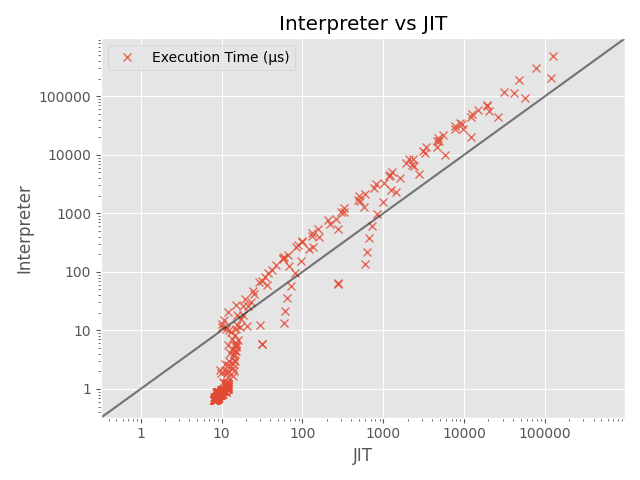
\includegraphics[scale=0.75]{output/graphs/scatter/vs/JIT-vs-Interpreter-time.png}
    \caption{Execution time of all tests for the JIT against the interpreter.}
    \label{figure:time-jit-interpreter}
\end{figure}

\begin{figure}[H]
    \centering
    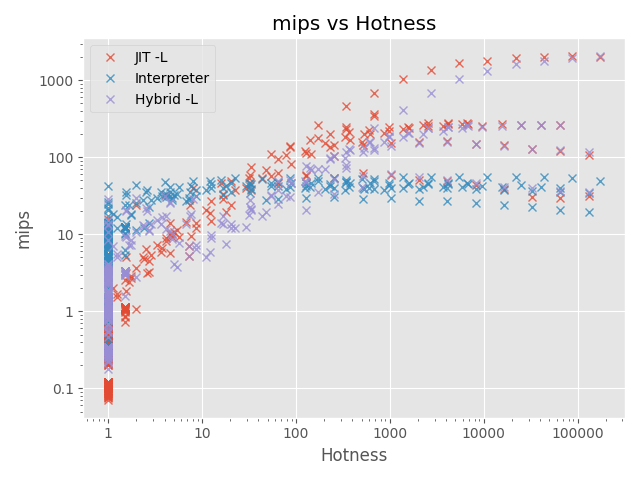
\includegraphics[scale=0.75]{output/graphs/scatter/emulators/hotness.png}
    \caption{Performance against hotness for all tests.}
    \label{figure:hotness}
\end{figure}

\subfile{interpreter}
\subfile{jit}
\subfile{hybrid}
\subfile{iteration}
\subfile{recursion}
\subfile{memory}
